\section{Domain Informed Oracle} 
\subsection{Architecture}
In this section, we lay the foundations of the architecture that combines the Domain Informed Oracle with 
reinforcement learning. Note that in our proposed architecture, we suppose Proximal Policy Optimization, a specific method to compute the policy in RL that is explained in more details in \ref{sec:rldetails}. 
It does not mean that our solution is specific to it, rather it can be generalized to any algorithm choice.

\medskip 

\begin{figure}[H]
  \centering
  \begin{minipage}{.5\textwidth}
    \centering
    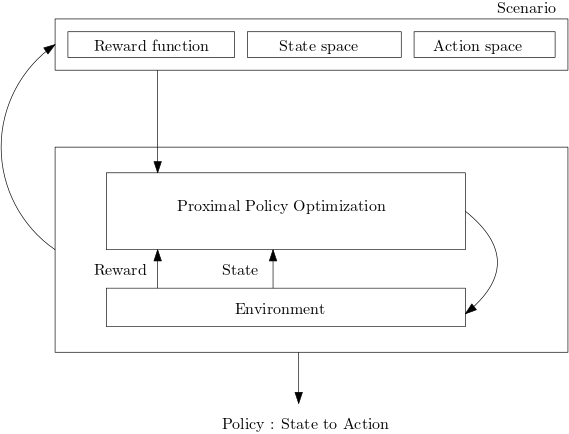
\includegraphics[width=1\linewidth]{figures/basicrl.png}
    \captionof{figure}{Reinforcement learning architecture}
    \label{fig:basicrl}
  \end{minipage}%
  \begin{minipage}{.45\textwidth}
    \centering
    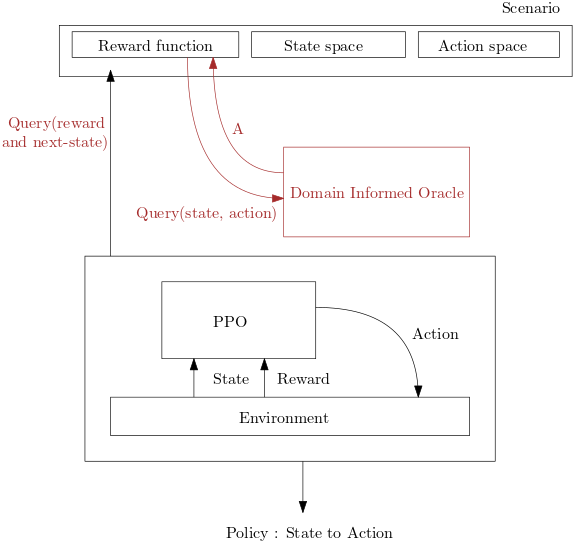
\includegraphics[width=1\linewidth]{figures/dio.png}
    \captionof{figure}{\dio+RL architecture}
    \label{fig:diorl}
  \end{minipage}
\end{figure}


The diagram in Figure \ref{fig:basicrl} describes the basic routine of RL in more details. The environment defined by the scenario sends the current state 
to the Q-Learning algorithm. The agent chooses an action from the action space and sends it to the environment. This action affects the environment stepping it to some next state. 
The resulting state along its associated reward is computed from the reward function and step function formalized in the scenario. Thus, in the next iteration, the 
agent receives the reward from its previous action which it uses to improve its policy and continues with its training starting from the computed next state.  

\medskip 

The architecture in Figure \ref{fig:diorl} introduces \dio in the feedback loop. It is kept independent of the RL module. Precisely, when the scenario is query-ed for the reward and 
the resulting next state of a (state, action) pair, rather than computing the reward using the reward function, the latter is able to query \dio. The result of this query is $A$ which we keep 
obscure. The fundamental idea is that $A$ is used to inform the reward function when it is tasked with computing the reward. 
 

\subsection{\dio procedure}
\label{sec:modules}
In practice, we consider the following modules and their interactions as shown in \ref{fig:mods}.

\begin{enumerate}
  \item \textbf{World Rules} defining the rules governing the world. This is domain-dependent and implemented 
        in a logic programming file, i.e. we are able to define the next step via step semantics.
  \item \textbf{Knowledge Base} defining the ground facts which describe the world at a given time step. This module is 
        continuously updated to account for the dynamics of the
        state.
  \item \textbf{Labels} i.e., textual ``norms'' corresponding to an
  iteration of the state. In practice, they are all possible judgments on the resulting state, e.g. \textit{crash :- obs(X,Y), agent(X,Y)}, 
                  or \textit{maybecrash :- nextObs(X,Y), agent(X,Y)}. 
                    Those labels have probabilities associated with
                    them.
  \item \textbf{Translation Unit} defining the translation from state to ground facts and from labels to a numerical value, e.g. if the predicate crash is true with $P = 0.25$, then the reward shaped is $r + -0.25$. 
  \item \textbf{Reinforcement Learning} is our independent module that does not make assumption on the algorithm chosen for RL.
\end{enumerate}


\begin{figure}[H]
  \centering
  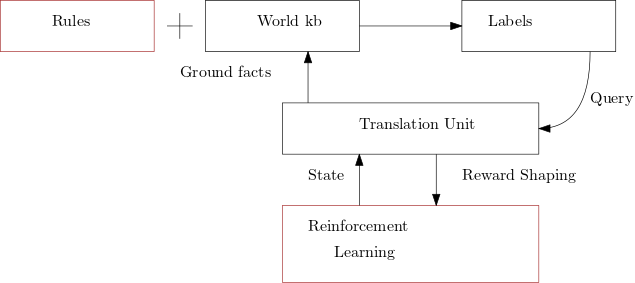
\includegraphics[scale=0.55]{figures/dynamics.png}
  \caption{Modules \& Interactions}
  \label{fig:mods}
\end{figure}

Figure \ref{fig:mods} describes the interactions of the different modules, basically taking a closure look to \dio. Precisely, 
given the rules and the world knowledge base at a given time $t$, we are able 
to produce the corresponding label, i.e. the query over a predicate. The predicate is fed 
into the Translation Unit (TU) that transforms the predicate to a numerical value that is given to the Reinforcement Learning 
as a reward shaping $r'$. This new reward can either \emph{overwrite} the previous reward, or \emph{fine-tune it}. In general, 
the way this reward affects the initial reward is a \textbf{design choice} that we leave for future investigations. 
Finally, as a result of the RL action, the next state is given 
to TU that translates it into Ground facts to update the world
knowledge, thus restarting the loop. Note that the inference on the query is done by a declarative tool that incorporates 
probabilities called \emph{Problog} that we introduce in \ref{sec:problog}.


\subsection{Problog Procedure} 
\label{sec:problog}
% High level overview of Problog
Problog is a logic programming language that aims to bridge between probabilistic 
logic programming and statistical relational learning \cite{fierens_van}. 
A problog program specifies a probability distribution over possible worlds. 
This probability distribution corresponds to the possible worlds whether a fact is taken 
or discarded given the probability associated with it. Precisely, they define a world 
is a subset of ground probabilistic facts where the probability of the subset is the product of 
the probabilities of the facts it contains.

\paragraph{Statistical Relational Learning (SRL)}
    Discipline of Artificial Intelligence that considers first order logic relations between 
    structures of a complex system and model it through probabilistic graphs such as Bayesian or 
    Markov networks.

\paragraph{Probabilistic Logic Programming (PLP)}
    Discipline of Programming Languages that augments traditional logic programming such as Prolog 
    with the power to infer over probabilistic facts to support the modeling of structured 
    probability distributions.


% Evidence and inference tasks in Problog
\paragraph{}
Furthermore, problog extends PLP with the power of considering evidences 
in the inference task. This is made possible without requiring the transformation 
the Bayesian networks on which to use SRL. Instead, problog considers the subset described above 
and assumes only worlds where the evidence held remains true. Those possible worlds and their associated 
probabilities are then added and divided by the choice with the higher probability. Problog makes this 
possible by a 3-steps conversion from a problog program to a weighted boolean formula.

\paragraph{}
% Conversion steps to weighted formula
First, problog grounds the program by only considering facts relevant to the query in question. 
The relevant ground rules are specifically converted to equivalent Boolean formulas. 
Precisely, inferences are converted into bi-directional implications and its corresponding premises 
are converted to a conjunction of disjunction of facts. 
Finally, problog asserts the evidence by adding it to the previous boolean formula 
as a conjunction and defines a weight function that assigns a weight to every literal. 
The weights are derived from the probability associated with the relevant literal, whether explicility 
given or implicility computed. 

